\section{Tvorba hry}

\subsection{Uživatelské rozhraní}
Program je postaven na grafické knihovně\\ JavaFX pro programovací jazyk Java. Vzhledem k povaze hry je JavaFX zcela 
dostačující.

\subsubsection{Struktura}
% TODO: Přidat obrázky rozhraní
Celé uživatelské rozhraní se nachází ve dvou oknech. V prvním okně (obrázek \ref{fig:okno1}) uživatel najde hru 
společně s časovačem a dvěma až třemi tlačítky. Autosweeper lze používat jen s tímto jedním oknem, ale kdyby chtěl
uživatel změnit nastavení hry, může tak učinit ve druhém okně (obrázek \ref{fig:okno2}), které otevírá tlačítko
"settings". V nastavení lze změnit velikost pole, pravděpodobnost min a herní mód. Druhé okno je možné mít otevřené
pořád, nastavení se přenese vždy jen do příští hry, kterou začneme zmáčknutím smajlíku. Smajlík v prvním okně také
slouží jako indikátor stavu hry. (obrázek \ref{fig:stavy smajlíku})

    \begin{itemize}
        \item Okno 1
        \begin{itemize}
            \item Tlačítko se smajlíkem na restart hry, indikátor stavu hry
            \item Tlačítko na otevření nastavení
            \item Tlačítko na analýzu v módu s pomocí
            \item Herní pole
            \item Časovač
        \end{itemize}
        \item Okno 2
        \begin{itemize}
            \item Posuvník upravující šířku pole
            \item Posuvník upravující výšku pole
            \item Posuvník upravující pravděpodobnost výskytu min
            \item Tlačítko s výběrem herních módů
        \end{itemize}
    \end{itemize}

\begin{figure}
    \centering
    
\includegraphics[scale=0.6]{smiley.png}
    \caption{Všechny stavy smajlíku. Popisky (zleva): Neutrální, Prohra, Hráč odhaluje minu, Výhra}
    \label{fig:stavy smajlíku}
\end{figure}

\begin{figure*}
    \centering
    \begin{subfigure}[b]{0.3\textwidth}
        \centering
        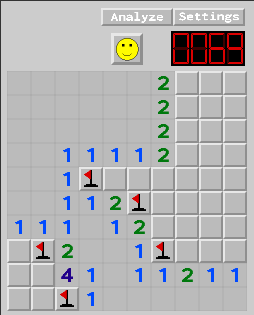
\includegraphics[scale=0.5]{images/okno1.png}
        \caption{Hlavní okno}
        \label{fig:okno1}
    \end{subfigure}
    \begin{subfigure}[b]{0.3\textwidth}
        \centering
        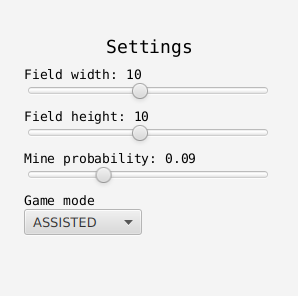
\includegraphics[scale=0.5]{images/okno2.png}
        \caption{Okno s nastavením}
        \label{fig:okno2}
    \end{subfigure}
    \caption{Okna s uživatelským rozhraním}
    \label{fig:okna}
\end{figure*}

\subsubsection{Design}
Vzhled programu je pokus o klon originálního designu Windows Minesweeper. Jako vzor byla použita jedna z mnoha
webových implemen-\\tací \autocite{playminesweeper}, jsou z ní vybrané zejména barvy čísel a vzhled smajlíku při
různých stavech hry. Původě mělo herní pole být tvořeno z několika tlačítek neboli objektů typu \\
{\tt javafx.scene.control.Button}, to by ale vyžadovalo hodně stylování a pravděpodobně také vytvořit si své
vlastní písmo s originálními číslicemi. Místo tlačítek jsou tedy využité \\{\tt javafx.scene.image.ImageView},
které umožňují zobrazit výstřižek obrázku. Na jednotlivé {\tt ImageView} jsou poté navázány funkce spouštějící
se při zmáčknutí, nebo puštění talčítka od myši.

Podobný problém nastal u časovače. Originálně byl jeho sedmi-segmentový displej generován, ale moderní
počítače mají dost paměti na to, aby mohla každá číslice být uložená jako obrázek. Každá viditelná cifra je
stejně jako u všeho ostatního jeden {\tt ImageView}, všechny jsou poté spravovány třídou \\{\tt SevenSegmentDisplay}.

Všechny obrázky byly tvořeny mnou v programu Aseprite.\footnote{Aseprite je placený, ale open-source. Je tedy zcela možné si
Aseprite zkompilovat zadarmo, což byla metoda, kterou jsem zvolil.}

\subsection{Herní pole a stav hry}
Herní pole je hlavní částí programu. Poté co ho ovladač hlavního okna vytvoří, spravuje celou hru. Při inicializaci
nového pole ({\tt PlayingField}) je třeba poskytnout jen herní nastavení. Pole poté vygeneruje všechna políčka,
které lze dostat zpátky pomocí metody {\tt getCellAt}. Aby bylo možné pole rychle vykreslit,
je implementována metoda {\tt render}, která jako parametr dostane JavaFX {\tt GridPane}, do kterého
vloží \\všechny políčka.

\subsubsection{Komunikace mezi herním polem a hlavním ovladačem}
Po inicializaci pole a zavolání metody {\tt render} se vše odehrává uvnitř nově vytvořeného objektu.
Pro snadnou komunikaci s hlavním ovladačem a zajištění reagování ostatních prvků v uživatelském rozhraní existuje
systém událostí. Ovladač může použít metodu {\tt setEventHandler} pro nastavení funkce, která bude
naslouchat \\událostem ve hře. Například pří začátku hry nastane událost typu {\tt EventType.START}. 
Naslouchající funkce tuto událost zachytí a zapne časovač. Další herní události jsou například při odhalování políčka,
odhalení miny (= prohra), nebo při výhře.

\subsubsection{Stav hry}
V samotném objektu herního pole není uloženo moc informací. Jsou v něm uložené jen odkazy na jednotlivé políčka,
celkový počet bomb a počet neodhalených políček. Poslední dvě informace jsou potřeba jen při vyhodnocování,
jestli je hra dohraná, či ne. Většina informací o stavu hry jsou v jednotlivých políčkách, což jsou objekty třídy
{\tt Cell} (která dědí z již zmíněné třídy {\tt ImageView}). Každé políčko ukládá svou pozici, jestli je bomba, nebo
označené. Má také speciální hodnotu {\tt solver\_flags}, která slouží automatu k ukládání informací z minulých tahů,
a mnoho metod pro ulehčení práce s polem v automatu, nebo při vyhodnocování počtu bomb v okolí políčka. 

Jedna z výhod ukládání si informací rovnou v políčkách, které dědí z {\tt ImageView}, je možnost automatické aktualizace v uživatelském roz-\\hraní. Také se s takovými objekty jako s celky velmi dobře pracuje v automatu.